\begin{activite}[Différentes représentations des fractions]

\begin{partie}[Premiers partages entre amis]
\begin{enumerate}
 \item Neuf barres de céréales sont à partager équitablement entre quatre enfants. Écris la part de chaque enfant sous la forme d'une somme d'un entier et d'une fraction.
 \item Douze gaufres au chocolat sont à partager entre dix enfants. Schématise de deux façons différentes ce partage. Écris la part de chaque enfant sous la forme d'une somme d'un entier et d'une fraction.
 \end{enumerate}
\end{partie}

\begin{partie}[Des partages de pizzas !]
Quatre amis (Adeline, Bertrand, Chloé et Daniel) ont commandé au total trois pizzas. La part de chacun sera identique.
\begin{enumerate}
 \item Dessine sur ton cahier ces trois pizzas et représente la part de chacun en supposant qu'ils mangent les pizzas les unes après les autres.
 \item On suppose maintenant que Bertrand doit manger en premier et ne réchauffer qu'une seule pizza. Dessine cette pizza et représente sa part.
 \item À l'aide des questions précédentes, trouve deux écritures différentes de la part de chacun et déduis‑en une égalité.
 \end{enumerate}
\end{partie}

\begin{partie}[Des tartes aux pommes et des baguettes !]
\begin{enumerate}
 \item Sami a invité neuf de ses amis pour son anniversaire. Il estime que lui et chacun d'entre eux mangeront un quart de tarte aux pommes. Combien de tartes aux pommes doit‑il commander ? Et s'il en invite finalement 11 ?
 \item Pour un pique‑nique organisé par le collège pour les classes de 6e, on estime que chacun des 155 élèves mangera un tiers de baguette. Combien de baguettes faut‑il alors prévoir pour ces élèves ? 
 \end{enumerate}
\end{partie}

\end{activite}

%%%%%%%%%%%%%%%%%%%%%%%%%%%%%%%%%%%%%%%%%%%%%%%%%%%%%%%%%%%%%%%%%%%%%%%%

\begin{activite}[Partages et comparaisons]

\begin{partie}
Axel vient de manger 4 carrés de chocolat sur une plaque qui en possède 24. Éloise vient d'en manger 3 sur une plaque de 18 carrés. La plaque de chocolat d'Éloise est identique à celle d'Axel.
\begin{enumerate}
 \item Représente sur la plaque de chocolat d'Axel, divisée en 24 carrés identiques ce qu'il a mangé ; \label{NbsRation_acti1}
 \item Effectue le même travail pour représenter ce qu'Éloise a mangé ; \label{NbsRation_acti2}
 \item En t'aidant des points \ref{NbsRation_acti1} et \ref{NbsRation_acti2}, détermine qui de Alex ou Éloise a mangé le plus de chocolat.
 \end{enumerate}
\end{partie}

\begin{minipage}[c]{0.78\linewidth}
\begin{partie}
Utilise le disque ci‑contre partagé en dix parts égales pour donner une fraction égale à $\dfrac{1}{2}$ Compare $\dfrac{1}{2}$ et $\dfrac{4}{10}$.
\end{partie}
\end{minipage} \hfill%
\begin{minipage}[c]{0.18\linewidth}
 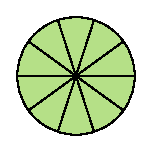
\includegraphics[width=2.1cm]{rond_vert}
 \end{minipage} \\

\begin{partie}
En utilisant maintenant un disque partagé en cent parts égales, compare $\dfrac{7}{10}$ et $\dfrac{3}{4}$.
\end{partie}

\begin{partie}
Donne une écriture décimale de chacune des fractions des questions précédentes.
\end{partie}

\end{activite}

%%%%%%%%%%%%%%%%%%%%%%%%%%%%%%%%%%%%%%%%%%%%%%%%%%%%%%%%%%%%%%%%%%%%%%%%

\begin{activite}[Quotients et demi‑droite graduée]

\begin{partie}
On a tracé ci‑dessous une demi‑droite graduée :
\begin{center} 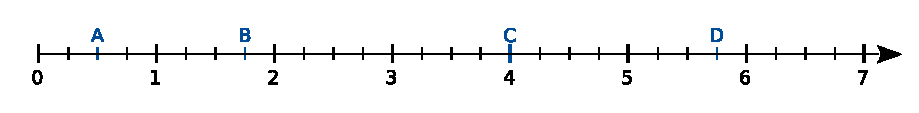
\includegraphics[width=15.5cm]{regle_ABCD07} \end{center}
\begin{enumerate}
 \item Donne de deux façons différentes les abscisses des points $A$, $B$, $C$ et $D$ ;
 \item Donne de deux façons différentes l'abscisse du point situé exactement au milieu des points $A$ et $B$ puis celui du point situé exactement au milieu de $C$ et $D$.
 \end{enumerate}
\end{partie}

\begin{partie}
Dessine une demi‑droite graduée et partage l'unité en 12 parts égales :
\begin{enumerate}
 \item Combien de ces parts faut‑il prendre pour avoir $\dfrac{1}{6}$ de l'unité ? Même question pour $\dfrac{1}{3}$, $\dfrac{1}{4}$ puis $\dfrac{1}{2}$ ;
 \item Place sur cette demi‑droite les points $E$, $F$, $G$ et $H$ d'abscisses respectives $\dfrac{13}{12}$, $\dfrac{2}{3}$, $\dfrac{3}{2}$ et $\dfrac{5}{4}$ ;
 \item Donne de deux façons différentes l'abscisse du point $K$ situé exactement au milieu de $G$ et $H$.
 \end{enumerate}
\end{partie}

\end{activite}

%%%%%%%%%%%%%%%%%%%%%%%%%%%%%%%%%%%%%%%%%%%%%%%%%%%%%%%%%%%%%%%%%%%%%%%%

\begin{activite}[Égalités de fractions]

\begin{partie}[De l'observation et de l'imagination \ldots]
On a représenté ci‑dessous trois fois le même rectangle avec la même surface coloriée. Chacun d'entre eux a été partagé en parts égales de différentes façons : \\[0.5em]
\begin{minipage}[c]{0.32\linewidth}
 \includegraphics[width=3.2cm]{surface_coloriee}
\end{minipage} \hfill%
\begin{minipage}[c]{0.32\linewidth}
 \includegraphics[width=3.2cm]{surface_coloriee2}
 \end{minipage} \hfill%
\begin{minipage}[c]{0.32\linewidth} 
 \includegraphics[width=3.2cm]{surface_coloriee3}
 \end{minipage} \\
\begin{enumerate}
 \item Pour chacun d'entre eux, quelle fraction du rectangle est coloriée en rose ? \label{NbsRatio_acti3}
 \item À l'aide de la question \ref{NbsRatio_acti3}, complète l'égalité suivante : $\dfrac{2}{3} = \dfrac{\ldots \ldots}{\ldots \ldots} = \dfrac{\ldots \ldots}{\ldots \ldots}$.
 \item En utilisant une méthode similaire, écris trois fractions égales à $\dfrac{10}{12}$.
 \item Est-il possible de trouver une fraction égale à $\dfrac{7}{9}$ ayant pour dénominateur 81 ? Ayant pour dénominateur 11 ? 
 \end{enumerate}
\end{partie}

\begin{partie}[Avec des demi-droites graduées (d'après IREM de Bordeaux)]
Décalque l'ensemble des demi-droites graduées ci‑dessous : \\[0.5em]
\begin{center} 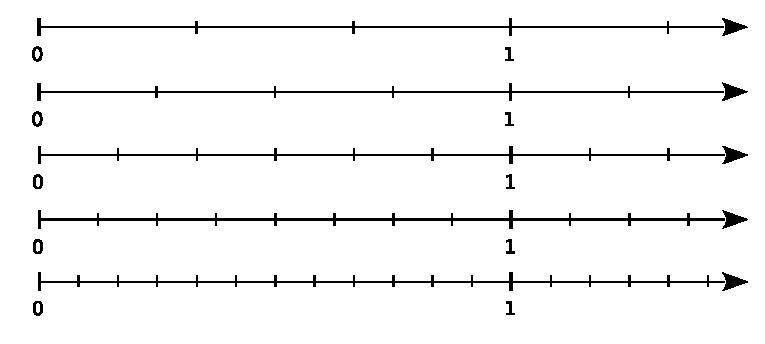
\includegraphics[width=13cm]{ddroites_graduees} \end{center}
\begin{enumerate}
 \item Choisis la demi‑droite graduée qui convient le mieux pour placer chacun des nombres suivants : $\dfrac{4}{3}$ ; $\dfrac{8}{6}$ et $\dfrac{16}{12}$. Que remarques‑tu ?
 \item Place $\dfrac{3}{4}$ sur la demi-droite graduée appropriée et déduis-en des fractions égales à $\dfrac{3}{4}$.
 \item En t'inspirant de ce qui précède, propose des fractions égales à 2 puis à 5.
 \end{enumerate}
\end{partie}

\begin{partie}[Avec la définition du quotient]
\begin{enumerate}
 \item Calcule les produits suivants :
 \begin{colitemize}{6}
  \item $2 \cdot 1,5$ ;
  \item $ 6 \cdot 1,5$ ; 
  \item $8 \cdot 1,5$ ;
  \item $10 \cdot 1,5$ ; 
  \item $12 \cdot 1,5$ ; 
  \item $22 \cdot 1,5$.
 \end{colitemize}
 \item À l'aide de la définition du quotient, déduis‑en des fractions égales à 1,5.
 \end{enumerate}
\end{partie}

\begin{partie}[Synthèse]
À l'aide de ce qui précède, détermine la condition pour que deux fractions soient égales.
\end{partie}

\begin{partie}[Des applications]
\begin{enumerate}
 \item Trouve une fraction « plus simple » (c'est-à-dire avec un \textbf{numérateur} et un \textbf{dénominateur} plus petits) égale à $\dfrac{35}{14}$ ;
 \item En détaillant ta démarche, détermine une fraction égale à $\dfrac{5,1}{0,75}$.
 
Simplifie, si possible, cette fraction.
 \end{enumerate}
\end{partie}

\end{activite}

%%%%%%%%%%%%%%%%%%%%%%%%%%%%%%%%%%%%%%%%%%%%%%%%%%%%%%%%%%%%%%%%%%%%%%%%

\begin{activite}[Comparaisons dans les cas simples]

\begin{center} 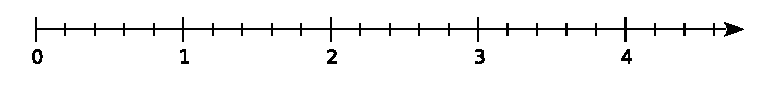
\includegraphics[width=12.6cm]{regle01234_bis} \end{center}

Lola la tortue et Jeannot le lapin décident de faire une course sur la demi-droite graduée ci-dessus. Le point de départ est l'origine de la demi-droite. Lola parcourt $\dfrac{7}{5}$ d'unité et Jeannot parcourt $\dfrac{12}{5}$ d'unité.

\begin{enumerate}
 \item Reproduis la demi-droite graduée ci-dessus puis places-y les points $L$ et $J$ pour indiquer les positions de Lola et de Jeannot. 
 \item Lequel des deux a parcouru le plus grand trajet ? Parmi les fractions $\dfrac{7}{5}$ et $\dfrac{12}{5}$, quelle est la plus grande ? \label{NbsRatio_acti4}
 \item En t'aidant de la question \ref{NbsRatio_acti4}, énonce une règle qui permet de comparer des fractions de même dénominateur. 
 \item Applique la règle que tu as trouvée pour comparer $\dfrac{25}{109}$ et $\dfrac{38}{109}$ puis $\dfrac{7,9}{23}$ et $\dfrac{7,09}{23}$.
\end{enumerate}

\end{activite}

%%%%%%%%%%%%%%%%%%%%%%%%%%%%%%%%%%%%%%%%%%%%%%%%%%%%%%%%%%%%%%%%%%%%%%%%

\begin{activite}[Comparaisons dans les cas complexes]

\begin{center} 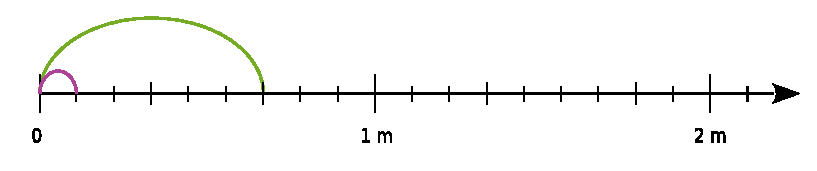
\includegraphics[width=13.5cm]{regle_kangourou} \end{center}

Zouzou le kangourou et Charlotte la puce décident de faire une course sur la demi-droite graduée ci-dessus. Le point de départ est l'origine de la demi-droite. Zouzou fait des bonds de $\dfrac{2}{3}$ de mètre (en vert) tandis que Charlotte fait des bonds de $\dfrac{1}{9}$ de mètre (en rose).

\begin{enumerate}
 \item Charlotte a fait 11 bonds tandis que Zouzou n'en a fait que 2. Reproduis la demi-droite graduée ci-dessus puis places-y les points $C$ et $Z$ pour indiquer les positions de Charlotte et de Zouzou. 
 \item Complète les phrases suivantes : \label{NbsRatio_acti5}
 \begin{itemize}
  \item « Charlotte a parcouru $\dfrac{\ldots \ldots}{9}$ de mètre. »
  \vspace{0.2cm}
  \item « Zouzou a parcouru $\dfrac{\ldots \ldots}{3}$ de mètre, ce qui équivaut à $\dfrac{\ldots \ldots}{9}$ de mètre. »
  \end{itemize}
  \vspace{0.2cm}
 \item En t'aidant de la question \ref{NbsRatio_acti5}, indique lequel des deux a parcouru le plus grand trajet. Parmi les fractions $\dfrac{11}{9}$ et $\dfrac{4}{3}$, quelle est la plus grande ? 
 \item Énonce une règle qui permet de comparer des fractions de dénominateurs différents.
 \item Applique la règle que tu as trouvée pour comparer $\dfrac{8}{3}$ et $\dfrac{39}{15}$ puis $\dfrac{2,1}{12}$ et $\dfrac{6,03}{36}$.
 \end{enumerate}

\end{activite}

%%%%%%%%%%%%%%%%%%%%%%%%%%%%%%%%%%%%%%%%%%%%%%%%%%%%%%%%%%%%%%%%%%%%%%%%

\begin{activite}[Prendre une fraction d'une quantité]

\begin{minipage}[c]{0.7\linewidth}
\begin{partie}[C'est pas de la tarte !]
\begin{enumerate}
 \item Florence a acheté une tarte de 400 g qu'elle a partagée en huit parts égales. Très gourmande, elle en a mangé les trois huitièmes. Calcule la masse d'une part de tarte et déduis-en la quantité, en grammes, mangée par Florence.
 \item Pour fêter son anniversaire, Patrice a acheté trois tartes identiques à celle de Florence.
 
À la fin de la fête, il annonce fièrement : « J'ai mangé le huitième des tartes ! ». Quelle quantité de tarte, en grammes, a‑t‑il mangée ?
 \item Quelle autre opération permet de retrouver les réponses précédentes ?
 
Complète alors : « Prendre les $\dfrac{3}{8}$ de 400 revient à \ldots ».
 \end{enumerate}
\end{partie}
\end{minipage} \hfill%
\begin{minipage}[c]{0.27\linewidth}
\begin{center} 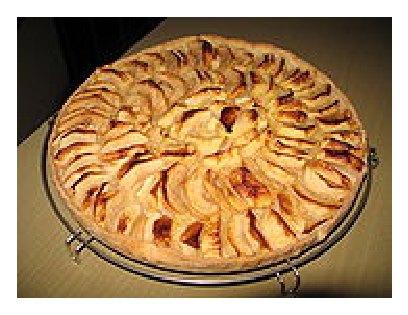
\includegraphics[width=4cm]{tarte_pommes} \end{center}
\begin{center} \quad \tiny{ \phantom{..}Copyleft Manuel Flury \newline \phantom{.........} Wikimedia commons \newline Licence GNU-FDL 1.2} \end{center}
\end{minipage} \\

\begin{partie}[Histoire de sous \ldots]
Mario devait 5 sésames (monnaie utilisée en Sésamathie, pays des sésamatheux) à Bastien. 
Comme il ne les a pas rendus en temps et en heure, Bastien lui réclame des intérêts en lui demandant maintenant de lui donner les sept tiers de cette somme.
\begin{enumerate}
 \item Mario se dit que « prendre 7 tiers de 5, c'est prendre 7 fois le tiers de 5. Or le tiers de 5, c'est le quotient de 5 par 3, soit exactement \ldots ». \\[0.5em]
Poursuis son raisonnement pour déterminer la somme exacte à rembourser.
 \item Complète : « Prendre les $\dfrac{7}{3}$ de 5 revient à \ldots ».
 \end{enumerate}
\end{partie}

\end{activite}

%%%%%%%%%%%%%%%%%%%%%%%%%%%%%%%%%%%%%%%%%%%%%%%%%%%%%%%%%%%%%%%%%%%%%%%%

\begin{activite}[Quelques applications]

\begin{partie}[Question de méthode !]
\begin{enumerate}
 \item Calcule chacun des produits suivants de trois façons différentes :
 \begin{colitemize}{3}
  \item $8 \cdot \dfrac{7}{4}$ ;
  \item $2,5 \cdot \dfrac{2}{5}$ ; 
  \item $ \dfrac{12}{6} \cdot 9$.
   \end{colitemize}
   \vspace{0.3cm}
Dans chaque cas, y a‑t‑il une méthode plus simple que les autres ? Explique.
 \item Pour trouver une écriture décimale exacte de $21 \cdot \dfrac{3}{7}$, Chloé affirme qu'on ne peut pas utiliser l'une des méthodes. A‑t‑elle raison ? Explique.
 \item Choisis la méthode qui te semble la plus astucieuse pour calculer les produits suivants :
 \begin{colitemize}{3}
  \item $1,89 \cdot \dfrac{100}{9}$ ;
  \item $15 \cdot \dfrac{2}{3}$ ; 
  \item $45 \cdot \dfrac{8}{4}$.
   \end{colitemize}
 \item On voudrait trouver la valeur exacte de $5 \cdot \dfrac{7}{3}$. Calcule ce produit en utilisant les trois méthodes. Quelle réponse donnerais‑tu à la question posée ?
 \end{enumerate}
\end{partie}

%%%%%%%%%%%%%%%%%%%%%%%%%%%%%%%%%%%
%%%%%%%%%%%%%%%%%%%%%%%%%%%%%%%%%%%
%MiseEnPage
%%%%%%%%%%%%%%%%%%%%%%%%%%%%%%%%%%%
\newpage
%%%%%%%%%%%%%%%%%%%%%%%%%%%%%%%%%%%
%%%%%%%%%%%%%%%%%%%%%%%%%%%%%%%%%%%


\begin{partie}[Multiplier par 0,1 ; par 0,01 ; \ldots]
\begin{enumerate}
 \item En remplaçant 0,1 par une fraction décimale, calcule $5,4 \cdot 0,1$.
 
De la même façon, calcule $0,791 \cdot 0,001$ puis $2\,009 \cdot 0,01$.
 \item Quelle autre opération peut‑on effectuer à la place d'une multiplication par 0,1 ? Par 0,01 ? Et par 0,001 ?
 \end{enumerate}
\end{partie}

\begin{partie}[Des conversions]
\begin{enumerate}
 \item Complète : $56,5 \text{cm} = 56,5 \cdot \ldots \text{cm} = 56,5 \cdot \dfrac{1}{\ldots} \text{m} = \bigg(56,5 \cdot \dfrac{1}{\ldots} \bigg) \text{m} =\dfrac{\ldots}{\ldots} \, \text{m} = \ldots \text{m}$.
 \item En reproduisant un raisonnement du même type, convertis 87,2 mm en m.
 \end{enumerate}
\end{partie}

\end{activite}

%%%%%%%%%%%%%%%%%%%%%%%%%%%%%%%%%%%%%%%%%%%%%%%%%%%%%%%%%%%%%%%%%%%%%%%%

\begin{activite}[Appliquer un taux de pourcentage]

\begin{partie}
Un commerçant consent une remise de 18 \% sur tous ses articles :
\begin{enumerate}
 \item Combien représente cette remise sur un article valant 100 CHF au départ ?
 
Même question pour un article valant 1 CHF, puis pour un article valant 135 CHF au départ.
 \item Par quel nombre faut-il multiplier le prix de départ d'un article (en CHF) pour connaître le montant de la remise (en CHF) ? (Tu donneras ce nombre sous la forme d'une fraction décimale).
 \item Complète : « Prendre 18 \% d'un nombre revient à \ldots . ».
 \end{enumerate}
\end{partie}

\begin{partie}
Dans un magasin, un article coûte 240 CHF. Calcule le montant de la remise lorsque celle‑ci est de 50 \%. Que remarques‑tu ? À quelle fraction du prix de cet article correspond cette remise ? Mêmes questions pour une remise de 25 \% puis de 75 \%.
\end{partie}

\begin{partie}
Dans un autre magasin, on accorde 16 \% de remise sur un article coûtant 300 CHF.

Détermine astucieusement le montant de cette remise.
\end{partie}

\end{activite}

%%%%%%%%%%%%%%%%%%%%%%%%%%%%%%%%%%%%%%%%%%%%%%%%%%%%%%%%%%%%%%%%%%%%%%%%
%%%%%%%%%%%%%%%%%%%%%%%%%%%%%%%%%%%
%%%%%%%%%%%%%%%%%%%%%%%%%%%%%%%%%%%
%MiseEnPage
%%%%%%%%%%%%%%%%%%%%%%%%%%%%%%%%%%%
\newpage
%%%%%%%%%%%%%%%%%%%%%%%%%%%%%%%%%%%
%%%%%%%%%%%%%%%%%%%%%%%%%%%%%%%%%%%

\begin{activite}[Additions et soustractions]

\begin{enumerate}
 \item Complète par des fractions les phrases suivantes :
 
 \begin{minipage}[c]{0.68\linewidth}
 \begin{itemize}
  \item L'aire de la région verte représente $\dfrac{3}{\ldots}$ de l'aire totale ;
  \vspace{0.3cm}
  \item L'aire de la région rose représente $\dfrac{1}{\ldots}$ de l'aire totale.
  \end{itemize}
  \end{minipage} \hfill%
  \begin{minipage}[c]{0.28\linewidth}
  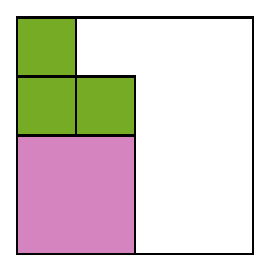
\includegraphics[width=3.6cm]{regions_vertesroses}
   \end{minipage} \\
 \item Écris le calcul à effectuer pour obtenir l'aire que représente la région coloriée par rapport à l'aire totale.
 \item Reproduis le carré ci-contre puis effectue des tracés judicieux pour obtenir ce que représente l'aire des deux régions verte et rose par rapport à l'aire totale. 
 \item Complète l'égalité suivante : $\dfrac{3}{16} + \dfrac{1}{4} = \dfrac{\ldots \ldots}{\ldots \ldots}$.
 \vspace{0.2cm}
 \item Que faudrait-il faire pour retrouver ce résultat par le calcul ?
 \item Énonce une règle qui permet d'additionner ou de soustraire des fractions de dénominateurs différents. 
 \item Applique la règle que tu as trouvée pour effectuer le calcul suivant : $\dfrac{2}{5} + \dfrac{1}{30}$.
\end{enumerate}

\end{activite}

%%%%%%%%%%%%%%%%%%%%%%%%%%%%%%%%%%%%%%%%%%%%%%%%%%%%%%%%%%%%%%%%%%%%%%%%
